\chapter{结论与展望}\label{ch:结论与展望}


\section{论文主要结论}\label{sec:论文主要结论}
\begin{itemize}
    \item \textbf{多条最短路问题相较于最短路问题提供了更多的可选方案}\\
    虽然大多数出行者往往会选择距离最短的路径出行,但对于不同出行者实际的路径选择仍然存在差异,
    不同出行者可能选择距离最短,时间最短,保证在指定时间前到达,经过红绿灯最少,必须经过指定某地等不同的实际需求。
    最短路算法仅仅考虑了将出行者的需求局限在路径最短的条件之下,既不能满足其它需求用户的需要,也不利于改善服务提供商的提供的服务。
    此外当路网系统某一结点或路段发生故障时,最短路径可能恰好失效,需要重新计算最短路。对于大规模路网中计算所需的时间是不可忽略的,会造成极其糟糕的用户体验。
    多条最短路作为最短路问题的拓展,既满足了出行者差异化的需要, 又为路网系统提供了高可靠性和高容错性,还使得服务提供商能为用户提供更好的服务。

    \item \textbf{基于偏离路径思想实现的k最短路寻路程序满足在线实时路径推荐系统的需要}\\
    在给出的多条最短路求解案例中,通过偏离路径的思想对比了手工求解和程序求解,验证了算法设计和程序设计的正确性。
    偏离路径实现实现的k最短路算法不仅可以获得精确的k条最短路,同时能保证最短路径中不存在环路,符合交通领域的实际需要。
    并且在小于100000个结点的路网中,基于偏离路径实现k最短路寻路程序和基于启发式规则实现了A-star寻路程序的执行效率相差不大,仅仅在超大规模路网中A-star算法相较于偏离路径算法的速度更快。
    但A-star算法所计算出的最短路径中会出现环路,对于交通领域实际应用场景而言相当于在某个区域\lq\lq{绕圈}\rq\rq, 在一般交通场景应用而言,默认求解的是无环的最短路径,
    因此使用A-star算法计算的最短路需要额外考虑去除带环路径,此外A-star算法的运行效率和启发式规则的选择有关,并且所求的最短路径是实际最短路径的近似解。

    \item \textbf{时间空间网络中最短路问题不满足Bellman条件,不能使用双向搜索算法加速}\\
    时间空间网络和静态网络不同的地方之一在于路段阻抗随时间变化,因此对于实际交通流的描述能力更强,尤其是对于不同时间节点路段阻抗差异较大的网络。
    若A到C的最短路径为A $\to$ P1 $\to$ B $\to$ C,则静态网络中可以得到A到B的最短路径为A $\to$ P1 $\to$ B,
    不同于静态网络,时间空间网络的最短路不满足Bellman条件,最短路不仅取决于两个结点之间的路段阻抗还和上一个结点的状态有关,故A到B的最短路径可能为 A $\to$ P2 $\to$ B。
    双向搜索算法加速最短路径的寻找需要知道源点和汇点的节点状态,而时间空间网络中的最短路为动态最短路,即需要知道上一个节点的状态才能知道下一个结点的状态,因此不适用双向搜索算法的使用条件。

    \item \textbf{时间空间网络在满足周期性变化的条件下可以转化为静态网络来简化处理}\\
    交通网络不同于一般的静态网络,交通流在早晚高峰时段和平峰时段的路段阻抗存在较大差异,路段阻抗属于时变属性集,因此交通网络属于时变网络。
    此外交通网络有着自己独特的流量特点,呈现周期性的变化特点,且在微观上交通流的变化是连续的,而在宏观上交通流的变化是离散的,呈现出双峰分布的特点。
    因此时间空间网络中的多条最短路问题可以通过时间拓展图的处理方法转化为静态网络中多个源点序列到多个汇点序列的多条最短路问题。
\end{itemize}


\section{论文创新点}\label{sec:论文创新点}
本文的创新点分为两个部分:
\begin{enumerate}%有序列表
    \item \textbf{在模型构建层面,考虑了除路段外的节点阻抗,并通过拆点的方法将路段阻抗和节点阻抗实现形式上的统一}\\
    在时间空间网络模型的构建过程中,不仅考虑了路段阻抗,同时还考虑了结点阻抗,增强了时间空间网络模型对各种交通行为的表示能力,例如在交叉口转向,或者在地铁换乘站换乘等行为。
    同时基于拆点的思想,将结点拆分为N-S, N-W, N-E, S-N, S-W, S-E, W-S, W-N, W-E, E-S, E-N, E-W等12个方向的路段,并根据路段通行能力对结点阻抗进行分配。

    \item \textbf{在算法设计层面,实现了时间空间网络下的多条最短路算法设计和分别实现了有环最短路和无环最短路寻路程序}\\
    对时间空间网络中k最短路算法的求解拆分为三个主要流程: 第一是对时间空间网络进行离散化处理;
    第二是通过设计程序对时间空间网络进行时间拓展表示,从而达到将时间空间网络转化为一般物理网络,实现对问题的等价转化;
    第三是通过在静态网络中的k最短路设计来实现程序,从而实现最终问题的求解。
    设计的处理k最短路程序在优化之后很好地符合交通领域问题研究的实际特点: 最短路径中无环路,计算A地到C地的最短路径中会自动排除掉了A地 $\to$ B地 $\to$A地 $\to$C地这种不符合实际场景的路径推荐。

\end{enumerate}


\section{研究展望}\label{sec:研究展望}
在时间-空间网络中k条最短路算法的设计中,根据交通流的周期性和微观连续性以及宏观离散性的特点来对时间-空间网络中路段阻抗函数进行离散化处理是关键一步。离散化处理需要根据交通流量的实际情况进行进一步确定,在未来的研究中,可以基于时间空间序列分析方法,大数据和机器学习中来实现阻抗的离散化处理和阻抗的动态预测。

机器学习作为一种以数据驱动的建模范式,其模型的建立可以通过借助计算机从海量数据中练习获得,进一步的减少研究者主观因素选择导致的模型不确定性。机器学习模型需要大数据的支持,而对于路段中无时无刻不在生成的交通流量数据尤为合适,因此机器学习建模在大数据时代有着无与伦比的先天优势。

数据驱动下的交通科学正在蓬勃发展。即使获取到了大量数据,但关键是找到利用数据的方法,利用数据为出行者提供更好的服务。显然多条最短路问题的研究是符合这一趋势的,并且问题本身有较强的研究价值和进一步的拓展空间。

%\begin{figure}[H] %H为当前位置,!htb为忽略美学标准,htbp为浮动图形
%    \centering %图片居中
%    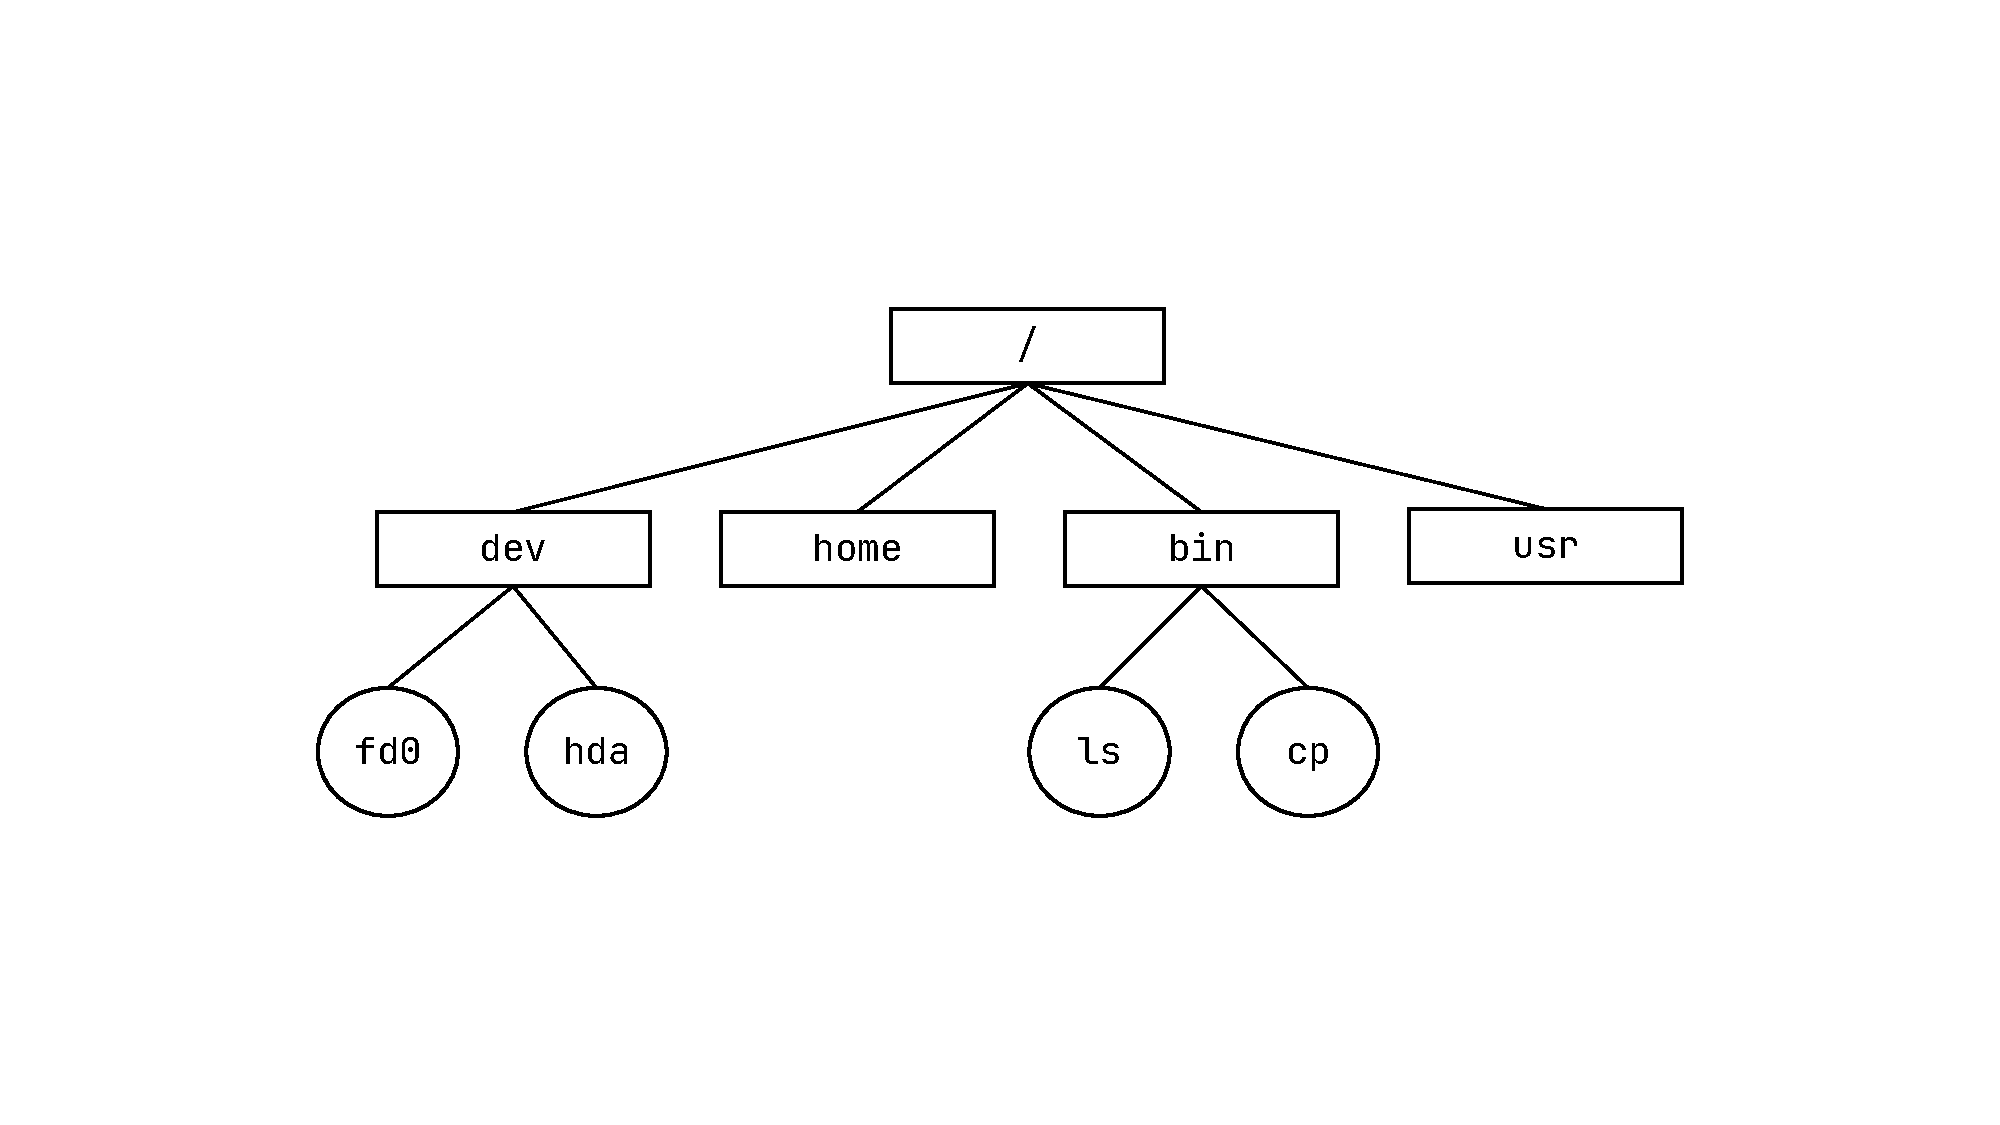
\includegraphics[width=0.7\textwidth]{png/book} %插入图片,[]中设置图片大小,{}中是图片文件名
%    \caption{book} %最终文档中希望显示的图片标题
%    \label{figx} %用于文内引用的标签
%\end{figure}
%如图\ref{figx}所示
